\section{lg\-Object Class Reference}
\label{classlgObject}\index{lgObject@{lgObject}}
a GUIDO object with no additional specific info  


{\tt \#include $<$lgobject.h$>$}

Inheritance diagram for lg\-Object::\begin{figure}[H]
\begin{center}
\leavevmode
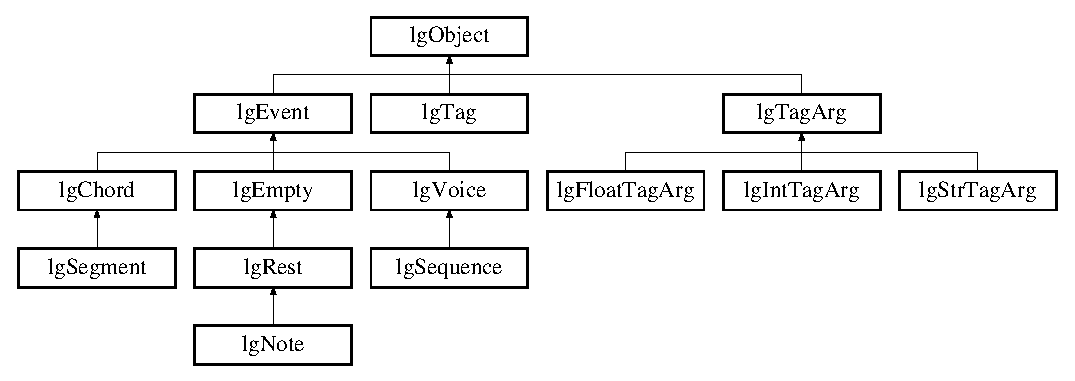
\includegraphics[height=4.66667cm]{classlgObject}
\end{center}
\end{figure}
\subsection*{Public Member Functions}
\begin{CompactItemize}
\item 
void {\bf accept} ({\bf string\-Visitor} v)
\item 
{\bf lg\-Object} $\ast$ {\bf next} (void)
\item 
{\bf lg\-Object} (void)
\item 
virtual string {\bf to\-String} ({\bf lg\-Voice} $\ast$calling\-Seq=NULL)
\item 
virtual void {\bf write} (FILE $\ast$out, {\bf lg\-Voice} $\ast$=NULL)
\begin{CompactList}\small\item\em write in GUIDO Syntax \item\end{CompactList}\item 
virtual {\bf lg\-Duration} {\bf pos} (void)
\end{CompactItemize}
\subsection*{Protected Member Functions}
\begin{CompactItemize}
\item 
virtual void {\bf set\-Next} ({\bf lg\-Object} $\ast$ptr)
\end{CompactItemize}
\subsection*{Protected Attributes}
\begin{CompactItemize}
\item 
{\bf lg\-Object} $\ast$ {\bf next\-I}
\end{CompactItemize}
\subsection*{Friends}
\begin{CompactItemize}
\item 
class {\bf lg\-Event}
\item 
class {\bf lg\-Voice}
\item 
class {\bf lg\-Sequence}
\item 
class {\bf lg\-Segment}
\item 
class {\bf lg\-Tag}
\item 
class {\bf lg\-Chord}
\end{CompactItemize}


\subsection{Detailed Description}
a GUIDO object with no additional specific info 



\subsection{Constructor \& Destructor Documentation}
\index{lgObject@{lg\-Object}!lgObject@{lgObject}}
\index{lgObject@{lgObject}!lgObject@{lg\-Object}}
\subsubsection{\setlength{\rightskip}{0pt plus 5cm}lg\-Object::lg\-Object (void)}\label{classlgObject_a2}




\subsection{Member Function Documentation}
\index{lgObject@{lg\-Object}!accept@{accept}}
\index{accept@{accept}!lgObject@{lg\-Object}}
\subsubsection{\setlength{\rightskip}{0pt plus 5cm}void lg\-Object::accept ({\bf string\-Visitor} {\em v})}\label{classlgObject_a0}




Reimplemented in {\bf lg\-Tag} {\rm (p.\,\pageref{classlgTag_a4})}.\index{lgObject@{lg\-Object}!next@{next}}
\index{next@{next}!lgObject@{lg\-Object}}
\subsubsection{\setlength{\rightskip}{0pt plus 5cm}{\bf lg\-Object}$\ast$ lg\-Object::next (void)\hspace{0.3cm}{\tt  [inline]}}\label{classlgObject_a1}


\index{lgObject@{lg\-Object}!pos@{pos}}
\index{pos@{pos}!lgObject@{lg\-Object}}
\subsubsection{\setlength{\rightskip}{0pt plus 5cm}virtual {\bf lg\-Duration} lg\-Object::pos (void)\hspace{0.3cm}{\tt  [inline, virtual]}}\label{classlgObject_a5}




Reimplemented in {\bf lg\-Event} {\rm (p.\,\pageref{classlgEvent_a6})}, and {\bf lg\-Tag} {\rm (p.\,\pageref{classlgTag_a25})}.\index{lgObject@{lg\-Object}!setNext@{setNext}}
\index{setNext@{setNext}!lgObject@{lg\-Object}}
\subsubsection{\setlength{\rightskip}{0pt plus 5cm}void lg\-Object::set\-Next ({\bf lg\-Object} $\ast$ {\em ptr})\hspace{0.3cm}{\tt  [protected, virtual]}}\label{classlgObject_b0}


\index{lgObject@{lg\-Object}!toString@{toString}}
\index{toString@{toString}!lgObject@{lg\-Object}}
\subsubsection{\setlength{\rightskip}{0pt plus 5cm}virtual string lg\-Object::to\-String ({\bf lg\-Voice} $\ast$ {\em calling\-Seq} = NULL)\hspace{0.3cm}{\tt  [inline, virtual]}}\label{classlgObject_a3}


get GUIDO string should be redefined in all derived classes 

Reimplemented in {\bf lg\-Chord} {\rm (p.\,\pageref{classlgChord_a6})}, {\bf lg\-Empty} {\rm (p.\,\pageref{classlgEmpty_a0})}, {\bf lg\-Event} {\rm (p.\,\pageref{classlgEvent_a1})}, {\bf lg\-Note} {\rm (p.\,\pageref{classlgNote_a0})}, {\bf lg\-Rest} {\rm (p.\,\pageref{classlgRest_a0})}, {\bf lg\-Segment} {\rm (p.\,\pageref{classlgSegment_a21})}, {\bf lg\-Sequence} {\rm (p.\,\pageref{classlgSequence_a0})}, {\bf lg\-Tag} {\rm (p.\,\pageref{classlgTag_a5})}, {\bf lg\-Tag\-Arg} {\rm (p.\,\pageref{classlgTagArg_a0})}, {\bf lg\-Str\-Tag\-Arg} {\rm (p.\,\pageref{classlgStrTagArg_a0})}, {\bf lg\-Int\-Tag\-Arg} {\rm (p.\,\pageref{classlgIntTagArg_a0})}, {\bf lg\-Float\-Tag\-Arg} {\rm (p.\,\pageref{classlgFloatTagArg_a0})}, and {\bf lg\-Voice} {\rm (p.\,\pageref{classlgVoice_a20})}.\index{lgObject@{lg\-Object}!write@{write}}
\index{write@{write}!lgObject@{lg\-Object}}
\subsubsection{\setlength{\rightskip}{0pt plus 5cm}virtual void lg\-Object::write (FILE $\ast$ {\em out}, {\bf lg\-Voice} $\ast$ = NULL)\hspace{0.3cm}{\tt  [inline, virtual]}}\label{classlgObject_a4}


write in GUIDO Syntax 



Reimplemented in {\bf lg\-Chord} {\rm (p.\,\pageref{classlgChord_a7})}, {\bf lg\-Event} {\rm (p.\,\pageref{classlgEvent_a8})}, {\bf lg\-Segment} {\rm (p.\,\pageref{classlgSegment_a22})}, and {\bf lg\-Voice} {\rm (p.\,\pageref{classlgVoice_a21})}.

\subsection{Friends And Related Function Documentation}
\index{lgObject@{lg\-Object}!lgChord@{lgChord}}
\index{lgChord@{lgChord}!lgObject@{lg\-Object}}
\subsubsection{\setlength{\rightskip}{0pt plus 5cm}friend class {\bf lg\-Chord}\hspace{0.3cm}{\tt  [friend]}}\label{classlgObject_n5}




Reimplemented in {\bf lg\-Event} {\rm (p.\,\pageref{classlgEvent_n1})}, {\bf lg\-Tag} {\rm (p.\,\pageref{classlgTag_n0})}, and {\bf lg\-Voice} {\rm (p.\,\pageref{classlgVoice_n0})}.\index{lgObject@{lg\-Object}!lgEvent@{lgEvent}}
\index{lgEvent@{lgEvent}!lgObject@{lg\-Object}}
\subsubsection{\setlength{\rightskip}{0pt plus 5cm}friend class {\bf lg\-Event}\hspace{0.3cm}{\tt  [friend]}}\label{classlgObject_n0}


\index{lgObject@{lg\-Object}!lgSegment@{lgSegment}}
\index{lgSegment@{lgSegment}!lgObject@{lg\-Object}}
\subsubsection{\setlength{\rightskip}{0pt plus 5cm}friend class {\bf lg\-Segment}\hspace{0.3cm}{\tt  [friend]}}\label{classlgObject_n3}




Reimplemented in {\bf lg\-Voice} {\rm (p.\,\pageref{classlgVoice_n1})}.\index{lgObject@{lg\-Object}!lgSequence@{lgSequence}}
\index{lgSequence@{lgSequence}!lgObject@{lg\-Object}}
\subsubsection{\setlength{\rightskip}{0pt plus 5cm}friend class {\bf lg\-Sequence}\hspace{0.3cm}{\tt  [friend]}}\label{classlgObject_n2}


\index{lgObject@{lg\-Object}!lgTag@{lgTag}}
\index{lgTag@{lgTag}!lgObject@{lg\-Object}}
\subsubsection{\setlength{\rightskip}{0pt plus 5cm}friend class {\bf lg\-Tag}\hspace{0.3cm}{\tt  [friend]}}\label{classlgObject_n4}


\index{lgObject@{lg\-Object}!lgVoice@{lgVoice}}
\index{lgVoice@{lgVoice}!lgObject@{lg\-Object}}
\subsubsection{\setlength{\rightskip}{0pt plus 5cm}friend class {\bf lg\-Voice}\hspace{0.3cm}{\tt  [friend]}}\label{classlgObject_n1}




Reimplemented in {\bf lg\-Event} {\rm (p.\,\pageref{classlgEvent_n0})}, and {\bf lg\-Tag} {\rm (p.\,\pageref{classlgTag_n1})}.

\subsection{Member Data Documentation}
\index{lgObject@{lg\-Object}!nextI@{nextI}}
\index{nextI@{nextI}!lgObject@{lg\-Object}}
\subsubsection{\setlength{\rightskip}{0pt plus 5cm}{\bf lg\-Object}$\ast$ {\bf lg\-Object::next\-I}\hspace{0.3cm}{\tt  [protected]}}\label{classlgObject_p0}




The documentation for this class was generated from the following files:\begin{CompactItemize}
\item 
{\bf lgobject.h}\item 
{\bf lgobject.cpp}\end{CompactItemize}
